\chapter{From Paper Figures to Talks and Posters}

In Chapter 9, Zhou, a doctoral student in materials science, finalized Figure 2 of his manuscript on interfacial passivation in perovskite solar cells. Designed as a double-column composite spanning $174\ \text{mm}$, the figure brings four panels together in a tight $2 \times 2$ grid: panel a diagrams the seven-layer planar device stack and highlights the ultrathin passivation layer; panel b shows a model-generated cross-sectional illustration of the layer morphology; panel c compares the current density--voltage ($J\text{--}V$) curves of the control and modified devices; and panel d tracks normalized power conversion efficiency (PCE) over $1000\ \text{h}$ of continuous illumination. Set uniformly in $8\ \text{pt}$ type with coordinated colours and line styles, the composite figure earned quick approval from his co-authors.

Two weeks later, however, Zhou has to present a 10-minute progress update at his department's joint group meeting, and a month after that he will bring an A0 portrait poster to an annual materials conference. Pressed for time, he takes a screenshot of Figure 2 from his manuscript PDF, drops the entire four-panel composite onto a 16:9 widescreen slide, and types a single word---``Results''---across the top (Figure~\ref{fig:ch12-05}a reproduces this exact slide at the visual angle experienced from the back row). When he projects the slide in the seminar room, labmates sitting in the last row squint at the screen and still cannot read the axis numbers. Worse, just as Zhou finishes walking through the layer stack in panel a and turns toward the efficiency curves, his advisor interrupts: ``Which curve in the bottom-left plot is the control? And did you take that cross-sectional electron micrograph in panel b yourself?'' Because the manuscript figure legend was left behind in the word processor and the in-panel labels blurred during rescaling, the audience can neither trace the curves nor tell that panel b is a conceptual illustration rather than experimental microscopy.

After the group meeting, Zhou turns to his conference poster. He copies the abstract, introduction, experimental methods, and conclusions from his manuscript into three dense columns of text and places an enlarged copy of Figure 2 dead center. When he sends a thumbnail preview to a senior postdoc in the lab, she replies with a single question: ``If a colleague walks down the poster aisle and glances at your board for five seconds, can they tell which interface you modified or how much the efficiency improved?''

Zhou's underlying scientific evidence has not changed at all. Why does a figure that works well in a journal manuscript fail so completely in a lecture hall and a poster session? The reason is that a journal page, a projected talk slide, and a conference poster board operate under three fundamentally different viewing conditions. Using the same perovskite interfacial-passivation study (built from simulated teaching data generated with a standard single-diode model), this chapter shows how to calculate readable font sizes and line weights from visual angles, how to unpack a multi-panel paper figure into a progressive sequence of 16:9 slides, how to structure an A0 portrait poster across three reading distances, and how to execute the redrawing, template layout, and cross-version consistency audit in \scidraw{}.

\section{One Study, Three Viewing Conditions}

When researchers prepare a conference talk or poster, they often treat the task as an exercise in compression---lifting paragraphs and composite figures straight out of a manuscript draft and squeezing them onto a new canvas. That habit overlooks a basic physical and cognitive reality. Reading a paper at a desk, watching slides in an auditorium, and browsing posters in an exhibition hall differ by orders of magnitude across three variables: \textbf{viewing distance, available time, and who controls the pace and bears the burden of explanation} (Figure~\ref{fig:ch12-01}).

\begin{figure}[htbp]\centering
\resizebox{\linewidth}{!}{% FIG ch12-01 three viewing conditions (English)
\begin{tikzpicture}[
  x=1mm, y=1mm,
  font=\sffamily\small,
  text=BookInk,
  coltitle/.style={font=\sffamily\bfseries, text=BookTeal, align=center},
  cell/.style={draw=BookRule, fill=white, align=left, text width=42mm, inner sep=2mm, minimum height=9mm},
  emphcell/.style={cell, fill=BookPale, draw=BookTeal, font=\sffamily\bfseries\small},
  icon/.style={draw=BookInk!40, fill=BookPale, line width=0.5pt},
]
  \foreach \x/\name/\w/\h in {22/Paper/42/59, 72/Talk/64/36, 122/Poster/42/59} {
    \begin{scope}[shift={(\x, 108)}]
      \node[coltitle] at (21, 14) {\name};
      \draw[icon, fill=white] (6, 0) rectangle ++(\w, \h);
      \ifnum\x=72
        \draw[BookInk!60, line width=0.8pt] (10, 4) -- (54, 4);
        \draw[BookInk!60, line width=0.8pt] (10, 32) -- (54, 32);
      \fi
    \end{scope}
  }
  \draw[BookTeal, line width=1pt] (10, 100) -- ++(20, 0);
  \node[font=\scriptsize, anchor=west] at (32, 100) {1 m (scale bar)};

  \node[cell, anchor=north west] at (0, 98) {Viewing distance};
  \node[cell] at (22, 89) {30--50 cm};
  \node[cell] at (72, 89) {2--15 m};
  \node[cell] at (122, 89) {First 2--5 m\\then 0.5--1.5 m};

  \node[cell, anchor=north west] at (0, 78) {Time available};
  \node[cell] at (22, 69) {Reader decides};
  \node[cell] at (72, 69) {About 1--2 min per slide};
  \node[cell] at (122, 69) {Seconds to stop\\minutes if staying};

  \node[cell, anchor=north west] at (0, 58) {Pace controlled by};
  \node[cell] at (22, 49) {Reader};
  \node[cell] at (72, 49) {Speaker};
  \node[cell] at (122, 49) {Viewer};

  \node[cell, anchor=north west] at (0, 38) {Who explains};
  \node[cell] at (22, 29) {Caption};
  \node[cell] at (72, 29) {Speaker};
  \node[cell] at (122, 29) {Poster itself};

  \node[emphcell, anchor=north west] at (0, 18) {Content strategy};
  \node[emphcell, text=BookTeal] at (22, 9) {Dense, self-contained};
  \node[emphcell, text=BookTeal] at (72, 9) {Sparse, sequential};
  \node[emphcell, text=BookTeal] at (122, 9) {Layered};
\end{tikzpicture}
}
\caption{Three viewing conditions. Distances and times are typical working values; check the actual venue and event requirements.}\label{fig:ch12-01}
\end{figure}

Start with the scale comparison at the top of Figure~\ref{fig:ch12-01}. When an A4 journal page ($210 \times 297\ \text{mm}$), a typical 16:9 auditorium projection screen (roughly $3.6\ \text{m}$ wide by $2.0\ \text{m}$ high), and an A0 portrait poster ($841 \times 1189\ \text{mm}$) are drawn to the same physical scale alongside a $1\ \text{m}$ reference bar, their surface areas span more than two orders of magnitude. Yet a larger canvas never entitles you to pack in more detail, because the viewer steps much farther back as the display grows.

\textbf{The first variable is viewing distance.} When reading a printed article or a PDF on a laptop screen, the eye sits roughly $30\text{--}50\ \text{cm}$ from the surface, and the reader can lean in to $25\ \text{cm}$ or zoom to $200\%$ whenever a label looks small. In an oral presentation, listeners sit $2\text{--}10\ \text{m}$ from the screen in a seminar room and $12\text{--}15\ \text{m}$ away in a large conference room, fixed in their seats. A poster hall introduces a two-stage geometry: attendees walking along the aisle scan boards from $2\text{--}5\ \text{m}$ away, step closer to $1\text{--}2\ \text{m}$ if a title or graphic catches their attention, and finally lean in to $0.5\text{--}1.5\ \text{m}$ to check experimental parameters.

\textbf{The second variable is available time.} A journal reader has unlimited time to compare panels a through d against the text and caption. In a live talk, a typical slide stays on screen for only $1\text{--}2\ \text{minutes}$ (a 10-minute slot holds roughly 8 to 10 content slides), and the audience must process the visual layout while simultaneously following spoken narration. Putting four sub-figures and dense text on screen at once forces visual search to compete with auditory comprehension. Poster sessions impose an even sharper filter: a passerby spends just a few seconds deciding whether to stop, and an interested visitor rarely stays longer than three to five minutes.

\textbf{The third variable is who controls the pace and explains the evidence.} In a paper, the \textbf{reader} controls the pace and relies on the \textbf{figure caption and main text} for explanation. In a talk, the \textbf{speaker} controls the clock and reveal sequence: listeners cannot flip back a slide or read your 200-word manuscript caption, so the speaker uses voice, pointer gestures, and step-by-step builds to supply context (Bourne, 2007; Naegle, 2021). At a poster session, control returns to the \textbf{viewer}, but because the presenter may be busy with another visitor or away from the board, a poster must be \textbf{self-explanatory} even when the author is absent (Erren and Bourne, 2007).

Taken together, these three variables dictate three distinct content-density strategies for the same study (bottom row of Figure~\ref{fig:ch12-01}):
\begin{itemize}
\item \textbf{Paper figures---dense and self-contained:} Short viewing distance, unconstrained time, and a full caption allow you to combine device architecture, morphology, primary performance, and stability data into one compact multi-panel figure for cross-panel comparison.
\item \textbf{Talk slides---sparse and sequential:} Long viewing distance, brief exposure per slide, and live narration require unpacking a composite figure across time: each slide answers one sub-question, pairing a single assertion headline with one piece of visual evidence.
\item \textbf{Conference posters---layered by distance:} As visitors move from the aisle to the board, the layout must stratify into three tiers: a top banner readable at $2\text{--}5\ \text{m}$ stating the question and main takeaway, three evidence blocks readable at $1\text{--}2\ \text{m}$ pairing assertion headings with redrawn plots, and a detail zone readable at $0.5\ \text{m}$ recording methods, parameters, and provenance notes.
\end{itemize}

Keep in mind that the distances and times in Figure~\ref{fig:ch12-01} represent typical working conditions rather than rigid regulations. Projection screen sizes in university defense rooms and poster board dimensions at international meetings vary widely; always check the conference's official presenter instructions or measure the room geometry before locking your canvas settings.

\section{Sizing Text by Visual Angle}

Once you recognize how viewing conditions shift across media, the most practical question immediately follows: ``What font size should I actually use on my slides and poster?'' Online advice columns routinely hand out fixed lookup tables---say, ``always use $24\ \text{pt}$ on slides and $28\ \text{pt}$ on posters.'' Yet presenting on an 85-inch wall monitor in a $5\ \text{m}$ seminar room is nothing like projecting onto a modest screen from $14\ \text{m}$ away in a raked lecture theater. Rather than memorizing rules of thumb, you can turn text sizing into a two-line geometric calculation that adapts to any room or poster hall.

Whether a human eye can comfortably resolve a printed or projected character does not depend on the character's absolute height $h$ in millimeters on the display surface; it depends on the \textbf{visual angle} $\theta$ that the character subtends at the retina. Whenever the viewing distance $d$ is much larger than the character height $h$, the small-angle approximation gives:
\[
\theta \approx \frac{h}{d}
\]
where $\theta$ is measured in radians (over the entire range of font sizes and viewing distances considered in this chapter, the small-angle approximation introduces an error below $0.1\%$). In plain terms, if you want a viewer standing ten times farther away to read a label as effortlessly as a reader holding a journal page, the physical height $h$ of the letters must scale up in direct proportion to the viewing distance $d$. In typography, font size is specified in points ($\text{pt}$), where $1\ \text{pt} = 1/72\ \text{in} \approx 0.3528\ \text{mm}$ (referring to the nominal height of the type body; both capital letter height and lowercase x-height scale linearly with point size). Once we anchor a comfortable baseline for desktop paper reading, we can compute the equivalent point size for any distance or screen geometry (Figure~\ref{fig:ch12-02}).

\begin{figure}[htbp]\centering
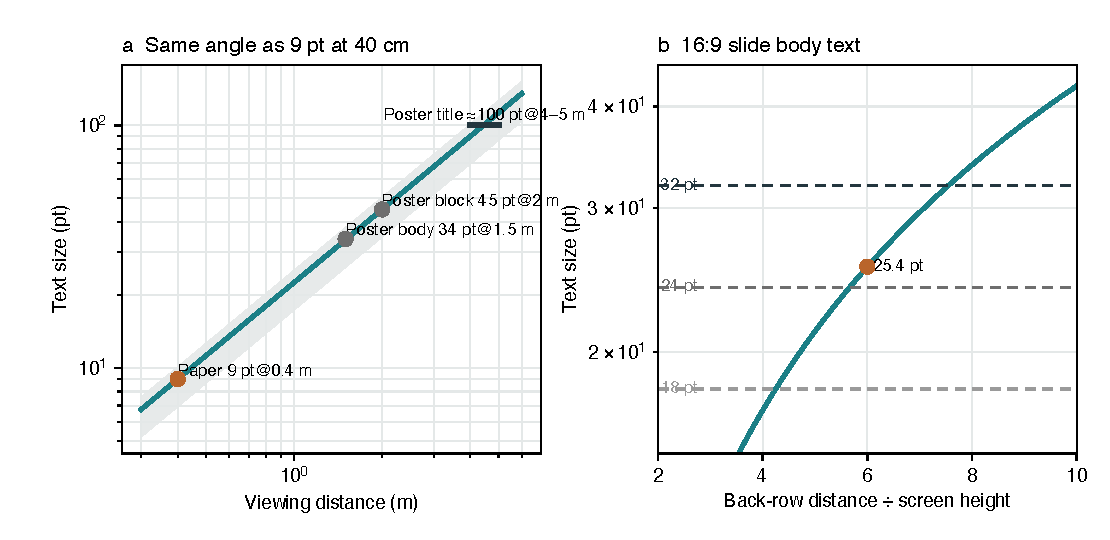
\includegraphics[width=\linewidth]{figures/ch12/ch12-02-visual-angle-text-size-en.pdf}
\caption{Text size from visual angle. Each curve gives the size that subtends the same angle as 9 pt text read at 40 cm. This is geometry, not a journal or conference rule; enlarge further for dim projection or less favourable viewing.}\label{fig:ch12-02}
\end{figure}

Let us walk through the four steps that produce the curves and benchmark markers in Figure~\ref{fig:ch12-02}.

\textbf{Step 1: Establish the desktop paper baseline.} When reading a printed journal issue or a tablet screen at a desk, a typical viewing distance is $d_0 = 40\ \text{cm} = 400\ \text{mm}$. A comfortable size for body text and clear figure annotations in print is $s_0 = 9\ \text{pt}$ (nominal body height $h_0 = 9 \times 0.3528 \approx 3.18\ \text{mm}$, with most journals setting $7\text{--}8\ \text{pt}$ as the lower floor for tick labels). Taking ``$9\ \text{pt}$ read at $40\ \text{cm}$'' as our reference benchmark gives a visual angle of:
\[
\theta_0 \approx \frac{3.18\ \text{mm}}{400\ \text{mm}} \approx 0.00794\ \text{rad} \approx 0.45^\circ
\]
If we translate the broader $7\text{--}10\ \text{pt}$ range common in published figures at $40\ \text{cm}$, the corresponding visual angle spans roughly $0.35^\circ\text{--}0.50^\circ$ (shown as the pale grey shaded band in Figure~\ref{fig:ch12-02}a). Note that ``$9\ \text{pt}$ at $40\ \text{cm}$'' is simply a convenient geometric reference chosen for mental arithmetic in this book, not a mandate from any publisher or standards body.

\textbf{Step 2: Scale poster text by physical viewing distance (Figure~\ref{fig:ch12-02}a).} Because an academic poster is laid out and printed at 1:1 physical dimensions (or at a known print scale factor), matching the visual angle of $9\ \text{pt}$ at $0.4\ \text{m}$ from a viewing distance $d$ (in meters) requires scaling the point size linearly with distance:
\[
s_{\text{poster}}(d) = 9 \times \frac{d}{0.4\ \text{m}}\ \text{pt} = 22.5\,d\ \text{pt}
\]
Substituting the three poster-hall viewing distances from Section 12.1 immediately yields target font sizes for the three information tiers:
\begin{itemize}
\item \textbf{Detail layer and close reading ($d = 1.0\text{--}1.5\ \text{m}$):} At $1.0\ \text{m}$, the equivalent size is $9 \times 1.0 / 0.4 = 22.5\ \text{pt}$; at $1.5\ \text{m}$---a natural distance when two or three colleagues stand side by side discussing a board---the equivalent size is $9 \times 1.5 / 0.4 = 33.75\ \text{pt} \approx 34\ \text{pt}$ (the lower grey dot in Figure~\ref{fig:ch12-02}a). Setting poster body bullets, axis titles, and tick labels between $28\ \text{pt}$ and $34\ \text{pt}$ ensures effortless reading at $1.5\ \text{m}$, while secondary methods notes and references meant for $0.5\text{--}1.0\ \text{m}$ inspection should never drop below $24\ \text{pt}$.
\item \textbf{Findings block headings ($d = 2.0\ \text{m}$):} So that a visitor standing two meters back or slightly down the aisle can grasp the takeaway sentence above each figure block at a glance, substituting $d = 2.0\ \text{m}$ gives $9 \times 2.0 / 0.4 = 45\ \text{pt}$ (the upper grey dot in Figure~\ref{fig:ch12-02}a).
\item \textbf{Top title banner ($d = 4.0\text{--}5.0\ \text{m}$):} To let passersby in the aisle read your research question from four to five meters away, substituting $d = 4.5\ \text{m}$ gives $9 \times 4.5 / 0.4 \approx 101\ \text{pt}$, spanning $90\text{--}113\ \text{pt}$ across the $4\text{--}5\ \text{m}$ interval (the dark horizontal bar near the top right of Figure~\ref{fig:ch12-02}a; notice how its text label \texttt{Poster title $\approx$100 pt@4--5 m} slightly crosses the right frame spine---a reminder to check label padding near plot borders).
\end{itemize}

\textbf{Step 3: Size slide text from the ratio of back-row distance to screen height (Figure~\ref{fig:ch12-02}b).} Projection slides differ from printed posters in one crucial respect: when you set type on a 16:9 slide in PowerPoint or Keynote, its physical height in the lecture hall depends entirely on the height $H$ of the venue's projection screen. Standard widescreen slide setups measure $13.333 \times 7.5\ \text{in}$ ($33.867 \times 19.05\ \text{cm}$), meaning the total vertical height of the slide canvas is fixed at $7.5 \times 72 = 540\ \text{pt}$. A font of nominal size $s_{\text{slide}}$ (in $\text{pt}$) therefore occupies a fraction $s_{\text{slide}} / 540$ of the screen height. If the physical screen height is $H$ and the back row sits at distance $D$, the visual angle subtended at the back row is:
\[
\theta \approx \frac{(s_{\text{slide}} / 540)\,H}{D} = \frac{s_{\text{slide}}}{540 \times (D/H)}
\]
Solving for $s_{\text{slide}}$ at our reference visual angle $\theta_0 \approx 0.45^\circ \approx 0.00785\ \text{rad}$ shows that the required slide font size depends only on the dimensionless ratio $D/H$ (back-row distance divided by screen height):
\[
s_{\text{slide}} \approx 0.00785 \times \left(\frac{D}{H}\right) \times 540\ \text{pt} \approx 4.24 \times \left(\frac{D}{H}\right)\ \text{pt}
\]
Two concrete examples show how this formula works in practice. First, consider a standard lecture hall with a screen height $H = 2.0\ \text{m}$ (width $\approx 3.56\ \text{m}$) and a back-row distance $D = 12\ \text{m}$, giving $D/H = 6$. On this screen, $24\ \text{pt}$ slide text occupies $24 / 540 = 1 / 22.5$ of the screen height ($\approx 8.9\ \text{cm}$ tall on the projection surface) and subtends $\approx 0.42^\circ$ at $12\ \text{m}$; matching $0.45^\circ$ exactly requires $25.4\ \text{pt}$ (the orange-brown dot in Figure~\ref{fig:ch12-02}b). This geometry explains a widely useful rule: \textbf{whenever the back row sits within roughly six screen heights of the display ($D/H \le 6$), $24\ \text{pt}$ is a safe floor for slide body text and axis titles, and tick labels should stay at or above $20\ \text{pt}$.}

Second, consider a long, low-ceilinged seminar room where the screen is only $H = 1.5\ \text{m}$ tall and the back table sits $D = 8\ \text{m}$ away ($D/H \approx 5.33$). If you drop figure labels to $18\ \text{pt}$ ($1/30$ of screen height), the visual angle at the back row shrinks to $(1.5 / 30) / 8 \approx 0.00625\ \text{rad} \approx 0.36^\circ$, right on the edge of the minimum legible floor in print. (As a practical graphic design note, inspect the left edge of Figure~\ref{fig:ch12-02}b: the reference labels \texttt{18 pt}, \texttt{24 pt}, and \texttt{32 pt} were placed flush against the left axis spine directly on top of the horizontal dashed lines; when labelling reference lines in your own charts, offset the text slightly above the dashed rule or into the right margin so the stroke never cuts through the numerals.)

\textbf{Step 4: Scale line weights and data markers in lockstep.} Visual angle governs curve strokes, axis spines, tick marks, and scatter symbols just as strictly as letterforms. On a printed journal page viewed at $40\ \text{cm}$, $0.5\text{--}0.8\ \text{pt}$ axis lines and $1.2\ \text{pt}$ data curves look crisp. Viewed from $1.5\ \text{m}$ on a poster, however, a $0.5\ \text{pt}$ hairline must be multiplied by $1.5 / 0.4 = 3.75$ to maintain the same apparent thickness. Data curves and axis spines on slides and posters should therefore be thickened to $2.0\text{--}3.5\ \text{pt}$. Whenever a room has a washed-out projector, strong ambient light, steep viewing angles from side aisles, or an international audience reading a second language, err on the side of larger type and heavier strokes than the bare geometric minimum.

\section{Turning a Paper Figure into a Slide Sequence}

With those geometric principles in hand, let us return to Zhou's perovskite solar cell study. We begin by inspecting the finalized manuscript version of Figure 2 from Chapter 9 (Figure~\ref{fig:ch12-03}) to see why a design that excels on a journal page breaks down when pasted onto a slide.

\begin{figure}[htbp]\centering
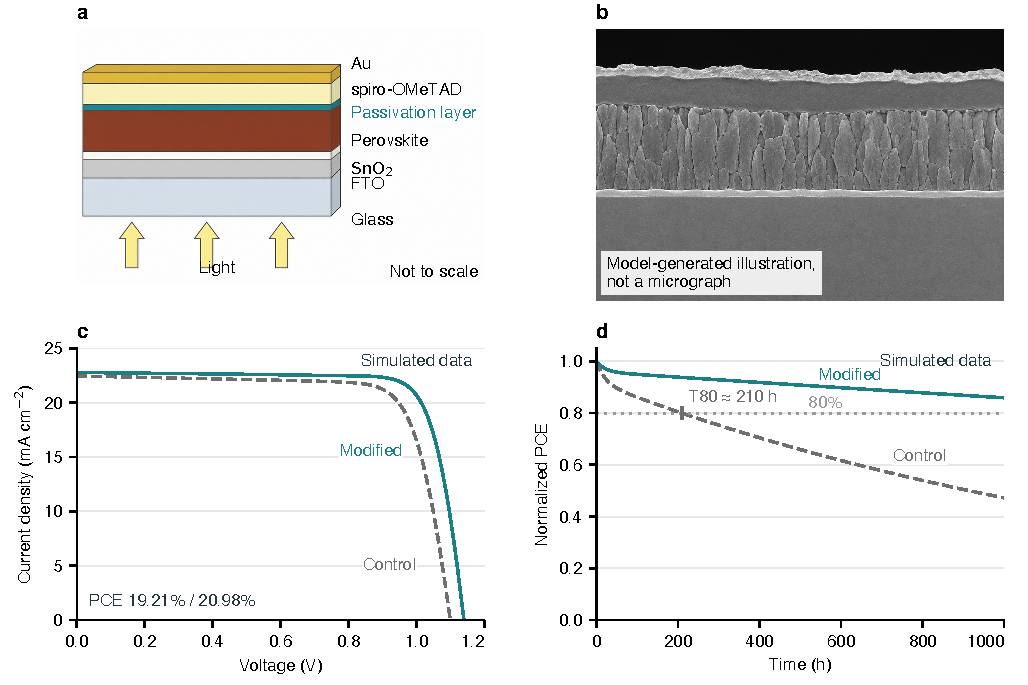
\includegraphics[width=\linewidth]{figures/ch12/ch12-03-paper-figure-2-en.pdf}
\caption{The paper version of Figure 2 (Chapter 9). Panels c and d show simulated data; panel b is a model-generated illustration, not a micrograph; panel a is not to scale.}\label{fig:ch12-03}
\end{figure}

In Figure~\ref{fig:ch12-03}, four panels fit cleanly inside a $174 \times 116\ \text{mm}$ double-column canvas: panel a diagrams the seven-layer stack ($\text{Glass}$, $\text{FTO}$, $\text{SnO}_2$, $\text{Perovskite}$, the teal $\text{Passivation layer}$, $\text{spiro-OMeTAD}$, and $\text{Au}$) with ``Not to scale'' at the bottom right; panel b shows a greyscale cross-sectional SEM-like texture with a light white box at the lower left explicitly stating ``Model-generated illustration, not a micrograph''; and panels c and d plot the simulated $J\text{--}V$ curves and $1000\ \text{h}$ normalized PCE stability traces using a grey dashed curve for the control device, a solid teal curve for the modified device, and ``Simulated data'' in the upper right corner. Yet when Zhou drops Figure~\ref{fig:ch12-03} wholesale onto a 16:9 slide and views it from the back row of the lecture hall, the audience sees Figure~\ref{fig:ch12-05}a.

\begin{figure}[htbp]\centering
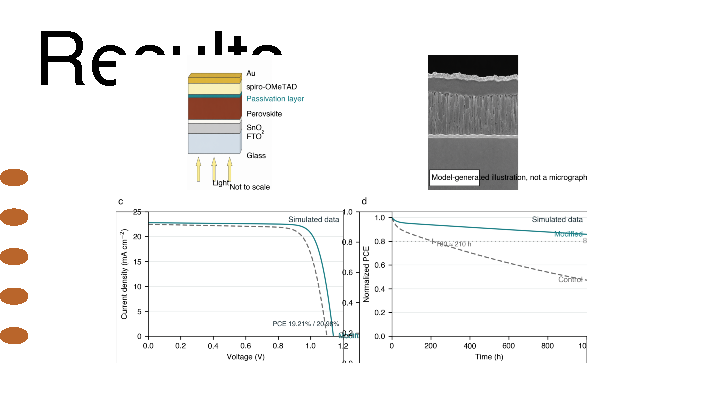
\includegraphics[width=119mm]{figures/ch12/ch12-05a-pasted-en.pdf}\\[1mm]
{\footnotesize (a) The paper figure pasted directly onto a slide: orange-brown markers (1)--(5) along the left margin flag the five defects analyzed in the text}\\[3mm]
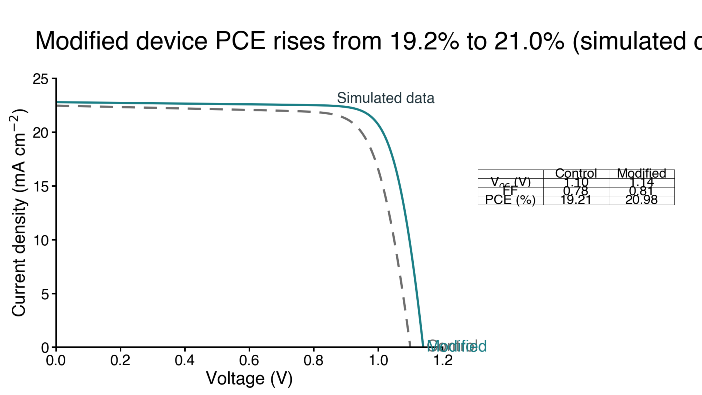
\includegraphics[width=119mm]{figures/ch12/ch12-05b-rebuilt-en.pdf}\\[1mm]
{\footnotesize (b) Slide 2b rebuilt for oral presentation: one question, an assertion headline, and large direct labels}
\caption{What the back row sees. Both slides are printed 119 mm wide; read at 40 cm, they subtend the same angle as a 3.6 m screen seen from 12 m. (a) The paper figure pasted in; (b) rebuilt for the talk. Simulated data.}\label{fig:ch12-05}\label{fig:ch12-05a}\label{fig:ch12-05b}
\end{figure}

The print width of Figure~\ref{fig:ch12-05} is calibrated to reproduce the exact visual angle of the back row: viewing a $3.56\ \text{m}$ wide 16:9 screen from $12\ \text{m}$ away subtends the exact same horizontal angle as viewing a $119\ \text{mm}$ wide image on this book page from $40\ \text{cm}$ ($3.56 / 12 \times 400\ \text{mm} \approx 119\ \text{mm}$). Held at normal reading distance, Figure~\ref{fig:ch12-05}a and Figure~\ref{fig:ch12-05}b show what a listener in row twelve actually experiences. Following the five orange-brown numbered circles (1)--(5) down the left margin of Figure~\ref{fig:ch12-05}a (notice that even the white numerals inside those margin circles are oversized and clipped by the circle borders), we can diagnose five concrete failures of the pasted-figure slide:
\begin{enumerate}
\item \textbf{Illegible tick labels and axis titles (marker 1):} Scaling a $174\ \text{mm}$ figure set in $8\ \text{pt}$ type (or a $180\ \text{mm}$ figure set in $7\ \text{pt}$ type) to $90\%$ of a 16:9 slide width ($\approx 305\ \text{mm}$) yields an effective slide font size of only $12\text{--}14\ \text{pt}$. At $12\ \text{m}$, those characters subtend just $0.21^\circ\text{--}0.25^\circ$---less than half the visual angle of normal paper reading---leaving the voltage and current-density scales unreadable from the back half of the room.
\item \textbf{Cramped annotations, colliding axes, and hard-to-trace curves (marker 2):} When a paper plot uses a corner legend box, listeners have to dart back and forth between legend keys and curves. Even when the paper plot uses direct labels, squeezing all four panels into a tight slide viewport causes severe collisions in Figure~\ref{fig:ch12-05}a: the right frame spine of panel c cuts straight through the vertical axis tick labels (\texttt{1.0}, \texttt{0.8}, \texttt{0.6}, \texttt{0.4}, \texttt{0.2}, \texttt{0.0}) of panel d; in the bottom-right corner of panel c, \texttt{Control} and \texttt{Modified} pile directly on top of each other and crash into the \texttt{1.2} tick mark; in panel d, \texttt{T80 $\approx$ 210 h} sits right across the grey dashed trace; and in panel a, \texttt{Light} collides with \texttt{Not to scale}.
\item \textbf{Four panels competing for attention at once (marker 3):} Projecting all four panels simultaneously splits the room's focus---while the speaker explains the $J\text{--}V$ sweep in panel c, half the audience is still deciphering the layer stack in panel a or squinting at panel b. Careless subplot placement also clips the outer edges: the top panel letters \texttt{a} and \texttt{b} are sliced off, and the rightmost horizontal tick \texttt{1000} in panel d is truncated to \texttt{10}.
\item \textbf{A topic label instead of a finding in the title bar (marker 4):} The heading \texttt{Results} in the upper left tells the audience nothing about what the study found (and in Figure~\ref{fig:ch12-05}a, the top of panel a's bounding box slices off the lower half of the word \texttt{Results}).
\item \textbf{Compromised or missing provenance disclosures (marker 5, highest integrity risk):} Because the manuscript figure legend is absent from the slide, the simulation conditions disappear. Worse, in panel b's lower-left disclaimer \texttt{Model-generated illustration, not a micrograph}, the white backing rectangle is too narrow, so \texttt{ed illustration, not a micrograph} spills out in black text across the dark grey cross-section and right margin, making it nearly invisible from the back row and inviting listeners to mistake a generative texture for an actual electron micrograph.
\end{enumerate}

Transforming Figure~\ref{fig:ch12-03} into a sequence of slides that read clearly from the back row (as in Figure~\ref{fig:ch12-05}b) follows a six-step workflow that converts spatial panels into a temporal narrative (Figure~\ref{fig:ch12-04}).

\begin{figure}[htbp]\centering
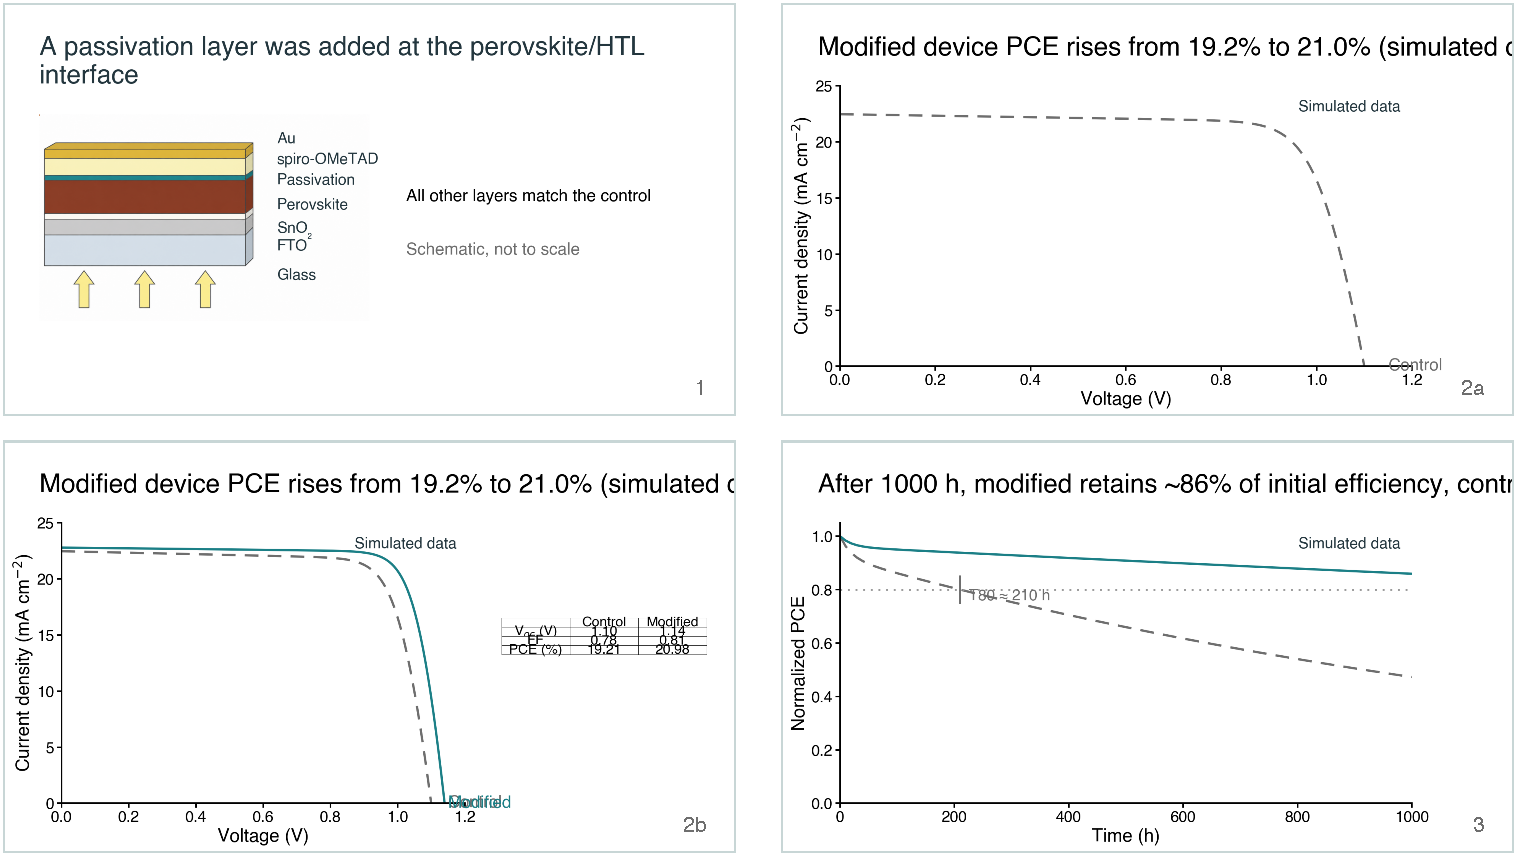
\includegraphics[width=\linewidth]{figures/ch12/ch12-04-slide-sequence-en.pdf}
\caption{Three talk slides built from the same data (slide 2 revealed in two steps). Each title states the finding, curves are labelled directly, and values, axis ranges and colour meanings match the paper figure. Simulated data.}\label{fig:ch12-04}
\end{figure}

\textbf{Step 1: List the sub-questions answered by the composite figure and move secondary panels to backup slides.} Figure 2 of the manuscript answers three sequential questions: (1) What physical change did we make to the device stack? (2) How much did that change raise initial photovoltaic efficiency? (3) How well did the modified device retain its efficiency over $1000\ \text{h}$ of operation? Because the cross-sectional illustration in panel b is a conceptual visual placeholder rather than primary quantitative evidence, it does not belong in the three-minute core talk flow; move it---together with its prominent ``Model-generated illustration, not a micrograph'' label---to a backup slide at the end of the deck for Q\&A.

\textbf{Step 2: Dedicate one slide to each sub-question and write an assertion headline.} Following the assertion--evidence structure widely used in scientific speaking (Naegle, 2021), replace generic headers like ``Results'' with a full $32\text{--}36\ \text{pt}$ sentence stating the takeaway and data status: Slide 1 reads ``A passivation layer was added at the perovskite/HTL interface''; Slide 2 reads ``Modified device PCE rises from $19.2\%$ to $21.0\%$ (simulated data)''; and Slide 3 reads ``After $1000\ \text{h}$, modified retains $\sim 86\%$ of initial efficiency, control $\sim 47\%$ (simulated data)''.

\textbf{Step 3: Use progressive reveal to pace complex comparisons.} Split Slide 2 into two identically registered frames (Slide 2a and Slide 2b in Figure~\ref{fig:ch12-04}). When Slide 2a first appears, only the axes and the grey dashed \texttt{Control} curve are visible, giving the speaker ten seconds to orient the room to the voltage and current-density scales. Advancing to Slide 2b (reproduced at back-row scale in Figure~\ref{fig:ch12-05}b) overlays the solid teal \texttt{Modified} curve on the exact same axis limits and reveals a compact summary table ($V_{\text{oc}}$, $\text{FF}$, and $\text{PCE}$) on the right. Because the axis bounding box never shifts between 2a and 2b, the eye immediately registers the outward expansion of the $J\text{--}V$ knee.

\textbf{Step 4: Strip away panel letters and detached legends in favor of direct callouts.} Delete the manuscript panel letters \texttt{a}--\texttt{d} and separate legend boxes. Label each curve directly by name, highlight the ultrathin passivation layer on Slide 1 with a bold orange-brown outline, and place just two short explanatory lines on the right of Slide 1 (``All other layers match the control'' and ``Schematic, not to scale'').

\textbf{Step 5: Redraw natively at 16:9 dimensions and audit the full-size export for text collisions.} Render every slide natively on a $13.333 \times 7.5\ \text{in}$ widescreen canvas (title $34\ \text{pt}$, axis titles $24\ \text{pt}$, tick labels $20\ \text{pt}$, annotations $22\ \text{pt}$, curve strokes $3\ \text{pt}$) rather than stretching a square or 4:3 plot. Crucially, always inspect the exported slides at full screen before walking into the seminar room. Examining the actual rendered frames in Figure~\ref{fig:ch12-04} and Figure~\ref{fig:ch12-05}b reveals four typographic flaws that an author must fix in presentation software or in the plotting script: (1) while Slide 1 wrapped its two-line title cleanly, the single-line $34\ \text{pt}$ titles on Slides 2a, 2b, and 3 are too long for the canvas width and get clipped at the right border (\texttt{... (simulated d} and \texttt{... contr})---insert a manual line break or reduce the title to $30\text{--}32\ \text{pt}$; (2) on Slides 2a and 2b (and Figure~\ref{fig:ch12-05}b), anchoring the direct labels \texttt{Control} and \texttt{Modified} to the final data point ($J = 0$) drops both words right onto the horizontal axis spine between $1.1\ \text{V}$ and $1.2\ \text{V}$ where they overwrite each other---move both labels upward into the open whitespace beside the steep descending knee of each curve; (3) on Slide 2b, the small summary table drawn by the plotting library has cramped vertical row height so \texttt{V\textsubscript{oc} (V)} and \texttt{FF} crowd the horizontal cell rules---building that three-row table natively in PowerPoint or Keynote gives much cleaner padding; and (4) on Slide 3, the \texttt{T80 $\approx$ 210 h} label sits directly across the grey dashed trace and the $0.8$ dotted reference line, and direct \texttt{Control}/\texttt{Modified} curve labels still need to be added above and below the traces.

\textbf{Step 6: Lock data values, axis ranges, colour semantics, and provenance notes across versions.} Keep every metric, axis range ($0\text{--}1.2\ \text{V}$, $0\text{--}25\ \text{mA cm}^{-2}$, $0\text{--}1000\ \text{h}$; if you ever zoom in on a sub-range, state that crop explicitly on the slide and in your spoken remarks), grey-dashed versus solid-teal encoding, and in-plot \texttt{Simulated data} tag identical to the manuscript figure.

\section{An A0 Portrait Poster: Grid, Hierarchy, and Density}

Under the ISO 216 international paper standard, an \textbf{A0 portrait poster} measures $841 \times 1189\ \text{mm}$---an area of exactly $1\ \text{m}^2$. Before dividing up that square meter of paper, consider how colleagues actually move through a conference poster hall (Figure~\ref{fig:ch12-07}).

\begin{figure}[htbp]\centering
\begin{tikzpicture}
\node[anchor=south west,inner sep=0] (img) at (0,0) {
\includegraphics[width=\linewidth]{figures/ch12/ch12-07-poster-hall-distances.png}};
\begin{scope}[x={(img.south east)},y={(img.north west)}]
  \node[font=\footnotesize,fill=white,fill opacity=0.88,text opacity=1,inner sep=2pt] at (0.18,0.12) {About 3--5 m: title and main finding};
  \node[font=\footnotesize,fill=white,fill opacity=0.88,text opacity=1,inner sep=2pt] at (0.58,0.12) {About 1 m: evidence and detail};
\end{scope}
\end{tikzpicture}
\caption{A poster is seen from afar before it is read up close. Illustration; figures and distances are not to scale (base illustration generated by an image model with distance labels overlaid by the author; prompts and generation records are available in the book repository).}\label{fig:ch12-07}
\end{figure}

When we generated the text-free base illustration for Figure~\ref{fig:ch12-07} from an English prompt, we ran the same prompt three times to get the spatial cues right: the first run drew the two faint dashed floor lines at sharply diverging angles, and the second run routed the outer dashed line behind the walking attendee's heels rather than beside their feet. The third run (Figure~\ref{fig:ch12-07}) aligned the two dashed floor lines with the two viewing positions---one passing the attendee walking down the aisle in the left foreground, the other passing just in front of the colleague standing close to the middle board---while keeping all five poster boards strictly abstract with teal/slate header bands, two-column grey rectangles, and unlabelled chart shapes (the row of boards spans roughly the right three-quarters of the frame with subtle soft shading, and the English distance callouts are overlaid in TikZ). That two-stage encounter---scanning from $3\text{--}5\ \text{m}$ in the aisle before stepping in to $1\ \text{m}$---governs every layout decision on an A0 poster (Figure~\ref{fig:ch12-06}).

\begin{figure}[htbp]\centering
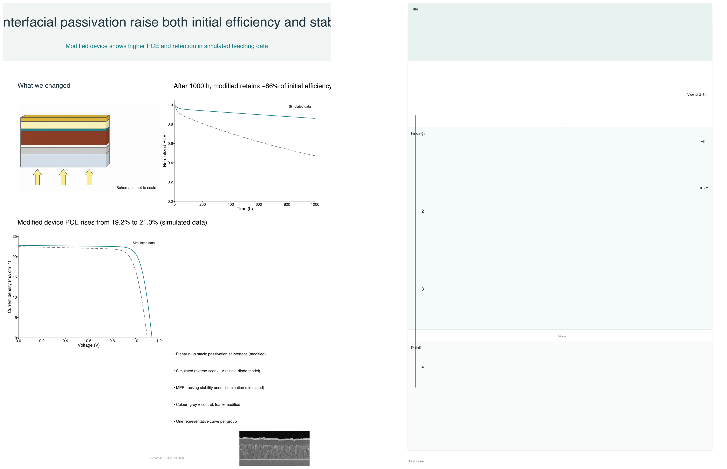
\includegraphics[width=\linewidth]{figures/ch12/ch12-06-a0-poster-layout-en.pdf}
\caption{An A0 portrait poster (841 $\times$ 1189 mm), final layout and wireframe. The three layers are written for reading at 3--5 m, 1--2 m and 0.5 m; plots were redrawn for viewing at 1.5 m. Simulated data; the cross-section is a model-generated illustration.}\label{fig:ch12-06}
\end{figure}

Comparing the rendered layout on the left of Figure~\ref{fig:ch12-06} with its structural wireframe on the right highlights three core design rules:
\begin{enumerate}
\item \textbf{A two-column grid with top-to-bottom column-wise reading order:} Leave a $30\ \text{mm}$ outer margin around all four edges (always $\ge 25\ \text{mm}$ so nothing is lost to printer bleed or poster-board clips), place a full-width $150\ \text{mm}$ title banner across the top, and divide the main body into two equal columns separated by a $20\ \text{mm}$ gutter (typically $15\text{--}20\ \text{mm}$), giving each column a net width of $380.5\ \text{mm}$. Organize the reading sequence vertically down the left column first (block 1 to block 2) and then down the right column (block 3 to block 4, following the vertical arrow on the wireframe), so a visitor standing in front of the board never has to zig-zag back and forth across nearly a meter of width after every panel (Erren and Bourne, 2007).
\item \textbf{Three distance tiers and a deliberate reassignment of the four manuscript panels:}
  \begin{itemize}
  \item \textbf{Title band (for $3\text{--}5\ \text{m}$ viewing):} Set inside a pale teal-grey banner at the top, the primary line asks the study question in $96\ \text{pt}$ type, while the second line states the main takeaway in $44\ \text{pt}$ teal type: ``Modified device shows higher PCE and retention in simulated teaching data''.
  \item \textbf{Findings layer (for $1\text{--}2\ \text{m}$ viewing):} Three large blocks occupy the upper and middle zones: top-left ``What we changed'' (device stack schematic M1 with a $28\ \text{pt}$ ``Schematic, not to scale'' note), bottom-left efficiency ($J\text{--}V$), and top-right operational stability. Each data block opens with a $48\ \text{pt}$ assertion heading above a plot redrawn specifically for $1.5\ \text{m}$ viewing (axis titles $32\ \text{pt}$, tick labels $28\ \text{pt}$, curve strokes $3.5\ \text{pt}$, and in-plot ``Simulated data'' note at $24\ \text{pt}$).
  \item \textbf{Detail layer (for $0.5\ \text{m}$ viewing):} The bottom-right zone groups five concise $28\ \text{pt}$ methodological bullets (planar n-i-p stack, single-diode reverse-scan model, MPP tracking condition, grey/teal colour key, and single representative curve notice) alongside a demoted thumbnail of panel b's cross-sectional illustration M2 carrying its $24\ \text{pt}$ provenance disclaimer.
  \end{itemize}
  Just as with the slides, inspecting the full-size A0 proof in Figure~\ref{fig:ch12-06} (left) at $100\%$ scale catches four layout items that must be cleaned up before sending the PDF to the print shop: (1) the centered $96\ \text{pt}$ question in the top banner (``Can interfacial passivation raise both initial efficiency and stability?'') exceeds the $841\ \text{mm}$ page width on a single line and gets clipped at both left and right margins (\texttt{nterfacial passivation raise both initial efficiency and stab})---wrap it onto two lines of $84\text{--}90\ \text{pt}$; (2) the $48\ \text{pt}$ assertion heading above the top-right stability block overflows the right margin (\texttt{... initial efficiency}) and needs a line break before ``control $\sim 47\%$''; (3) the device stack M1 and the two data plots need their $36\ \text{pt}$ layer names and direct \texttt{Control}/\texttt{Modified} curve labels added in the open canvas space; and (4) at the bottom edge of the M2 cross-section thumbnail in the lower-right corner, the dark text \texttt{Model-generated illustration, not a micrograph} sits directly over the dark grey substrate where it is clipped and hard to read---place it inside a light semi-transparent backing box just above the bottom edge.
\item \textbf{Density self-checks and the squint test:} Instead of aiming for an arbitrary word count, apply a five-minute reading test: can a colleague standing at $1.5\ \text{m}$ read every word on the poster in under five minutes while leaving generous open background around each plot? Then run the \textbf{squint test} (or thumbnail-and-blur test): shrink the poster to $12\ \text{cm}$ high and apply a Gaussian blur ($\sigma \approx 1.5\ \text{mm}$ at thumbnail scale) to simulate what the eye perceives from down the aisle (Figure~\ref{fig:ch12-08}).
\end{enumerate}

\begin{figure}[htbp]\centering
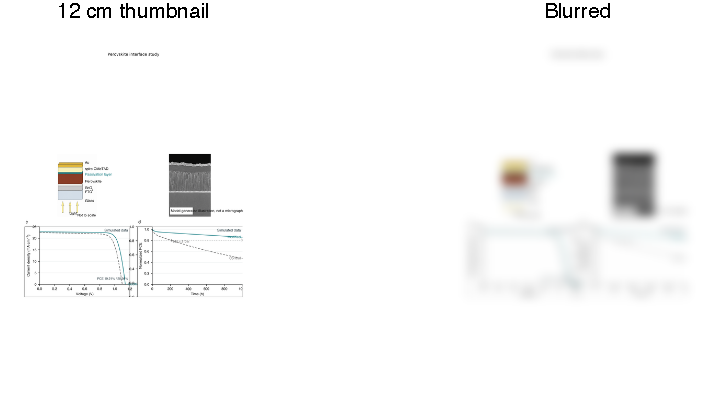
\includegraphics[width=\linewidth]{figures/ch12/ch12-08a-dense-squint-en.pdf}\\[1mm]
{\footnotesize (a) Crowded draft C0: three columns of manuscript prose above an enlarged copy of the four-panel paper figure}\\[3mm]
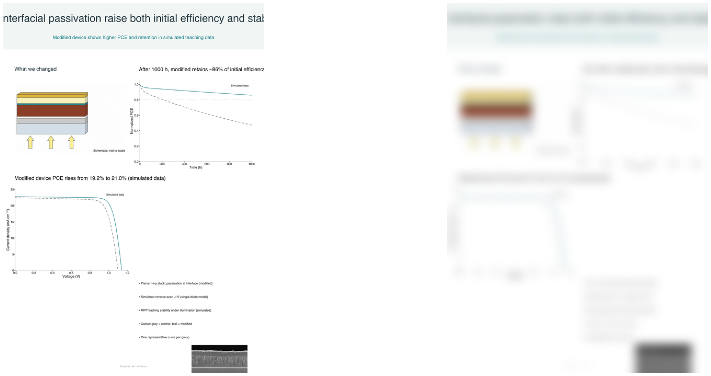
\includegraphics[width=\linewidth]{figures/ch12/ch12-08b-focused-squint-en.pdf}\\[1mm]
{\footnotesize (b) Layered final layout: top title banner, three findings blocks, and lower-right detail zone}
\caption{The squint test. Left: a 12 cm thumbnail; right: the same, blurred. (a) The crowded draft turns into an even grey; (b) the final layout keeps its title band and three blocks.}\label{fig:ch12-08}\label{fig:ch12-08a}\label{fig:ch12-08b}
\end{figure}

Compare Figure~\ref{fig:ch12-08}a and Figure~\ref{fig:ch12-08}b. In the crowded draft C0 (Figure~\ref{fig:ch12-08}a), the top of the board has only a small $36\ \text{pt}$ heading (\texttt{Perovskite interface study}) with no colored banner or main finding; the upper half is filled with five sections of $20\ \text{pt}$ manuscript prose across three columns (roughly 140 words in this sample mockup, which already fade to near-invisibility at $12\ \text{cm}$ thumbnail height); and the middle of the board simply enlarges the $174\ \text{mm}$ manuscript Figure 2 by roughly $4\times$ across the page (turning $0.6\ \text{pt}$ lines into $\sim 2.4\ \text{pt}$, which is passable, but scaling $8\ \text{pt}$ labels to $\sim 32\ \text{pt}$ with panels c and d still colliding, erasing any visual hierarchy between section headings and tick labels). Once blurred, C0 collapses into a featureless pale field above four indistinct smudges. In the layered final layout (Figure~\ref{fig:ch12-08}b), even after Gaussian blurring (and even with the un-wrapped top title line), the top banner, the three findings blocks with their bold assertion bars, and the bottom-right detail zone remain unmistakable.

\section{Completing All Three Versions in SciDraw AI}

When producing the manuscript figure, the slide sequence, and the conference poster in \scidraw{}, route each task to the workspace designed for it and keep a clear boundary between what the platform automates and what you must finish and verify in local software:
\begin{itemize}
\item \textbf{Redrawing data plots at new aspect ratios and font sizes (Scientific Visualization \sdtool{sci-vis}):} Rather than starting from scratch or re-uploading your CSV files, open the history session from your Chapter 9 manuscript plot, select the verified final version, and submit a targeted revision instruction to generate a 16:9 slide version, a control-only build frame for progressive reveal, and a thick-stroked poster panel. The workspace supports multi-turn conversational editing, branching from historical versions, restoring the previous or original state, and exporting in multiple formats. Afterward, verify that every numerical value, axis limit, and colour mapping remained intact, and check the actual rendered point size after placing the graphic onto your PowerPoint slide or A0 poster canvas (Chapter 13 examines how to verify whether an exported file contains true editable vector paths).
\item \textbf{Slide decks and poster layout frameworks (Presentation Templates \path{/scientific-presentation-templates} and Poster Templates):} The presentation template library provides downloadable 16:9 PPTX frameworks tailored for thesis defenses, conference talks, literature seminars, group meetings, and proposal defenses. The poster template library offers three layout families---Classic, Focus, and Four-Column---across standard academic dimensions including A0 portrait, A0 landscape, A1, $36 \times 48\ \text{in}$, $90 \times 120\ \text{cm}$, and 16:9 digital e-posters (note that $72\ \text{in}$ wide posters are built at $50\%$ physical dimensions to stay within presentation software page-size limits and are printed at $200\%$ scale, as noted inside the template file). Keep the boundary clear: \textbf{downloading a PPTX template does not automatically populate your content}. \scidraw{} does not offer a one-click tool that converts a manuscript into a multi-slide editable presentation or a print-ready editable poster; you assemble your redrawn plots and assertion headlines inside PowerPoint or Keynote.
\item \textbf{Exploring overall poster visual directions (Scientific Poster Maker \path{/scientific-poster-maker}):} This generator produces a single bitmap concept image of a poster from a text prompt, and can also draft a visual prompt by reading an uploaded manuscript PDF (currently parsing only the first five pages, abstract, and opening text rather than comprehending the full paper). Use it strictly as a rough mood board to compare column proportions or accent palettes before you start laying out your template. \textbf{Never send a generated poster bitmap to the printer as your final poster}, and never keep any text or synthetic ``charts'' rendered inside that bitmap; always build the real poster in an editable template or deterministic script using verified figures and text.
\item \textbf{Unpacking composite panels and checking target print width (Multi-Panel Figure Maker \sdtool{multi-panel-figure-maker} and Figure Checker \sdtool{figure-checker}):} When you export a composite figure as PPTX from \sdtool{multi-panel-figure-maker}, each panel bitmap and its panel letter (\texttt{a}, \texttt{b}, \dots) are stored as separate slide objects, making it easy to lift out the device schematic in panel a or delete the panel letters. However, the curves, axes, and labels inside each panel bitmap are not individually editable vector objects, so data panels still need to be redrawn at slide or poster font sizes in \sdtool{sci-vis} or your plotting script. Once assembled, run \sdtool{figure-checker} at your target physical width to audit effective resolution (ppi), greyscale contrast, and colour-vision deficiency risks---remembering that visual-angle legibility, reading order, and scientific accuracy remain the author's responsibility. Because tools do not automatically pipe files across workspaces, pass assets between stages by downloading clearly named files and importing them into the next step.
\end{itemize}

\section{Worked Case: One Study, Three Versions}

We now bring together the complete closed-loop record for our perovskite solar cell interfacial-passivation case: raw materials and simulation parameters, the three drawing briefs, copy-ready revision prompts, spoken narration and poster captions, and the cross-version consistency audit.

\textbf{1. Study setup and simulated data parameters.} This teaching case compares a planar n-i-p perovskite solar cell (control) against an otherwise identical stack incorporating an ultrathin interfacial passivation layer between the perovskite absorber and the hole transport layer (modified). No real experimental device measurements are reported; all numerical curves are generated deterministically from a standard single-diode equation and a two-term exponential decay model. Illuminated through the glass substrate, the stack sequence from bottom to top is: $\text{Glass}$ / $\text{FTO}$ / $\text{SnO}_2$ ($\sim 30\ \text{nm}$) / perovskite absorber ($\sim 500\ \text{nm}$) / interfacial passivation layer (modified group only, ultrathin) / $\text{spiro-OMeTAD}$ ($\sim 200\ \text{nm}$) / $\text{Au}$ back contact ($\sim 80\ \text{nm}$), without specifying a particular chemical formula for the perovskite composition or passivating molecule.

Across the four source materials, M1 is the layer-stack schematic (not to scale); M2 is a model-generated cross-sectional SEM-like texture (in an actual research paper, cross-sectional morphology must come from real electron microscopy of the same device batch with calibrated scale bars and unaltered raw backups as covered in Chapter 8; we use a generative texture here solely as a layout placeholder because no real micrograph exists for a simulated device, and every derived version must carry the explicit notice ``Model-generated illustration, not a micrograph''); M3 is the simulated reverse-scan $J\text{--}V$ dataset under AM1.5G illumination ($100\ \text{mW cm}^{-2}$) at $25\ ^\circ\text{C}$ solved from $J = J_L - J_0[\exp((V + J R_s)/(n V_T)) - 1] - (V + J R_s)/R_{\text{sh}}$ with $V_T = 0.025693\ \text{V}$ (a single scan direction is simulated without hysteresis; on $J\text{--}V$ hysteresis see Snaith et al., 2014, and on detailed-balance efficiency limits see Shockley and Queisser, 1961), where the control group ($J_L = 22.5\ \text{mA cm}^{-2}$, target $V_{\text{oc}} = 1.10\ \text{V}$, $n = 1.6$, $R_s = 2.5\ \Omega\cdot\text{cm}^2$, $R_{\text{sh}} = 1500\ \Omega\cdot\text{cm}^2$) yields $J_{\text{sc}} = 22.46\ \text{mA cm}^{-2}$, $V_{\text{oc}} = 1.100\ \text{V}$, $\text{FF} = 0.777$, and $\text{PCE} = 19.21\%$, and the modified group ($J_L = 22.8\ \text{mA cm}^{-2}$, target $V_{\text{oc}} = 1.14\ \text{V}$, $n = 1.5$, $R_s = 2.0\ \Omega\cdot\text{cm}^2$, $R_{\text{sh}} = 3000\ \Omega\cdot\text{cm}^2$) yields $J_{\text{sc}} = 22.78\ \text{mA cm}^{-2}$, $V_{\text{oc}} = 1.140\ \text{V}$, $\text{FF} = 0.808$, and $\text{PCE} = 20.98\%$; and M4 is the $0\text{--}1000\ \text{h}$ normalized PCE stability trace simulated for continuous 1-sun illumination with maximum-power-point (MPP) tracking in $\text{N}_2$ at $\sim 25\ ^\circ\text{C}$ (for consensus stability reporting protocols see Khenkin et al., 2020), where the control trace $y(t) = [1 - 0.08(1 - e^{-t/20})]e^{-t/1500}$ reaches $T_{80} = 210\ \text{h}$ and retains $0.47$ of its initial efficiency at $1000\ \text{h}$, while the modified trace $y(t) = [1 - 0.04(1 - e^{-t/20})]e^{-t/9000}$ stays above $0.80$ throughout the $1000\ \text{h}$ window ($T_{80} > 1000\ \text{h}$) and retains $0.86$ at $1000\ \text{h}$.

\textbf{2. The three drawing briefs.} Each version is governed by its own explicit brief before any redrawing begins.

Brief A (Manuscript Figure 2):
\begin{Prompt}
[Purpose & Audience] Manuscript Figure 2 for photovoltaic and materials peers;
read independently at ~40 cm; pace controlled by the reader.
[One-Sentence Goal] Readers can see that interfacial passivation improves both
initial efficiency and 1000 h stability over the control, and can locate Jsc,
Voc, FF, PCE, and T80.
[Panels] a device stack schematic; b cross-section texture (model-generated);
c simulated J-V curves; d simulated normalized PCE vs. time.
[Dimensions] Double-column 174 mm width, 8 pt in-panel labels, 10 pt bold
lowercase panel letters.
[Fixed Constraints] All values from the master metrics table; control = grey
#6E6E6E dashed, modified = teal #1B7F86 solid.
[Disclosures] Panels c, d labeled "Simulated data"; panel b labeled
"Model-generated illustration, not a micrograph"; panel a "Not to scale".
\end{Prompt}

Brief B (Group-meeting / conference talk sequence, 3 slides at 16:9):
\begin{Prompt}
[Purpose & Audience] 3-minute results segment in a 10-minute talk for group
members and materials peers; screen height ~2 m, back row 10-12 m; pace
controlled by the speaker.
[One-Sentence Goal] Listeners grasp in three sequential steps: what layer was
added -> how much initial efficiency rose -> how much 1000 h stability improved.
[Slide Plan]
  Slide 1 Title: "A passivation layer was added at the perovskite/HTL interface".
          Enlarged device schematic (M1) with passivation layer highlighted;
          cross-section texture M2 moved to backup slide with full disclaimer.
  Slide 2 Title: "Modified device PCE rises from 19.2% to 21.0% (simulated data)".
          Two-step reveal: (2a) axes + control curve; (2b) add modified curve +
          compact Voc/FF/PCE table; direct curve labels, no detached legend box.
  Slide 3 Title: "After 1000 h, modified retains ~86% of initial efficiency,
          control ~47% (simulated data)". Stability curves with 0.8 line & T80.
[Specs & Check] 16:9 (33.867 x 19.05 cm); ticks >= 20 pt, axis titles >= 24 pt,
slide titles 32-36 pt, lines >= 2.5 pt, no panel letters. Readable at 1/4 scale.
\end{Prompt}

Brief C (A0 portrait conference poster):
\begin{Prompt}
[Purpose & Audience] Conference poster hall, A0 portrait (841 x 1189 mm);
passersby scan from 2-5 m, visitors read at 0.5-1.5 m for 3-5 min; presenter
may not be present.
[One-Sentence Goal] Passersby read the question and main finding from 3 m;
closer visitors read "what changed -> efficiency -> stability" and key methods.
[Hierarchy] Title band: question + main finding (title >= 90 pt); Findings
layer: 3 blocks, each with an assertion heading (>= 44 pt) + redrawn figure;
Detail layer: 5 method bullets, M2 thumbnail + disclaimer (body >= 28 pt, min 24 pt).
[Grid & Order] 2 columns, 30 mm outer margin, 20 mm column gap; top-to-bottom
column-wise order: Banner -> Left-top (stack) -> Left-bottom (J-V) ->
Right-top (stability) -> Right-bottom (methods & M2 detail).
[Plots & Check] Redraw plots for 1.5 m viewing (ticks >= 28 pt, lines >= 3 pt).
Passes 12 cm blurred squint test and 1:1 A4 patch test at 1.5 m.
\end{Prompt}

\textbf{3. Copy-ready revision prompts and poster layout prompt.} Opening the Chapter 9 $J\text{--}V$ history session in \sdtool{sci-vis} and selecting the verified manuscript plot, submit the following revision instruction:
\begin{Prompt}
Keep all data points, both group colours (control #6E6E6E dashed, modified
#1B7F86 solid), the horizontal axis 0-1.2 V, and the vertical axis 0-25 mA/cm2
unchanged, and generate a version for a 16:9 presentation slide:
1. 16:9 canvas with the plot occupying roughly the left 60% of the frame;
2. Tick labels equivalent to 20 pt and axis titles 24 pt on a 33.867 cm wide
   slide; curve stroke width 3 pt;
3. Remove the legend box and label "Control" and "Modified" directly in the
   open space beside the descending knee of each curve (do not overlap y = 0);
4. Place "Simulated data" inside the upper right corner of the plot area;
5. Do not add any new numbers, error bars, or significance markers.
Also export a control-only frame with identical axis bounds for step-by-step reveal.
\end{Prompt}

After export, verify that the two reveal frames share identical pixel coordinates for the axis box so nothing jumps on click, confirm that every number matches the master metrics file, and check that the tool did not smooth the curves or alter the hex colours. To generate the poster $J\text{--}V$ plot, run the same prompt with item 2 adjusted to: ``For a $380\ \text{mm}$ wide block on an A0 poster viewed at $1.5\ \text{m}$: tick labels $28\ \text{pt}$, axis titles $32\ \text{pt}$, curve stroke width $3.5\ \text{pt}$.''

If you use \texttt{/scientific-poster-maker} to explore visual layout concepts before opening your PPTX template, use a text-free layout prompt:
\begin{Prompt}
A0 portrait academic poster layout for a materials science study, two columns,
clear title band across the top, three large figure blocks with generous white
space, a narrow footer band. Clean flat design, white background, one accent
color teal. Use simple placeholder rectangles for figures and grey bars for
text; do not render any readable words.
\end{Prompt}

\textbf{4. Spoken narration and poster block caption.} Accompanying spoken script for Slide 2 (Figure~\ref{fig:ch12-04}, transitioning from 2a to 2b in roughly 40 seconds):
\begin{BookNote}
``First look at the axes: horizontal is applied voltage from $0$ to $1.2\ \text{V}$, vertical is photocurrent density in $\text{mA cm}^{-2}$---the squarer the knee between the curve and the axes, the higher the fill factor. The grey dashed curve is our unpassivated control device---[advance slide]---and the solid teal curve is the interface-passivated device. Open-circuit voltage rises from $1.10\ \text{V}$ to $1.14\ \text{V}$, fill factor improves from $0.78$ to $0.81$, and power conversion efficiency increases from $19.2\%$ to $21.0\%$. Note that these curves are simulated teaching data used to illustrate the presentation workflow.''
\end{BookNote}

Accompanying short caption for the bottom-left $J\text{--}V$ block on the A0 poster:
\begin{BookNote}
The modified device shows higher open-circuit voltage and fill factor. Simulated reverse-scan $J\text{--}V$ curves (single-diode model), AM1.5G, $100\ \text{mW cm}^{-2}$; one representative curve per group, not a device-to-device distribution.
\end{BookNote}

\textbf{5. Cross-version consistency audit.} Before delivering the talk deck and sending the poster to print, audit all three versions row by row against Table~\ref{tab:ch12-02}.

\begin{table}[htbp]\centering\footnotesize
\setlength{\tabcolsep}{3pt}
\renewcommand{\arraystretch}{1.15}
\caption{Cross-version consistency audit across the manuscript figure, talk slides, and A0 poster.}\label{tab:ch12-02}
\begin{tabularx}{\linewidth}{@{}>{\raggedright\arraybackslash}p{26mm}YYY>{\raggedright\arraybackslash}p{18mm}@{}}
\toprule
\textbf{Audit item} & \textbf{Paper version} & \textbf{Slide version} & \textbf{Poster version} & \textbf{Consistent?} \\
\midrule
$J_{\text{sc}}$ / $V_{\text{oc}}$ / $\text{FF}$ / $\text{PCE}$ (both groups) & Master metrics table \& panel c callout & Slide 2 headline \& right-hand summary table & Bottom-left $J\text{--}V$ block heading \& plot & Exact match \\
$T_{80}$ (control $\approx 210\ \text{h}$) \& $1000\ \text{h}$ retention ($0.47$ / $0.86$) & Master metrics table \& panel d callout & Slide 3 headline \& in-plot callout & Top-right stability block heading \& plot & Exact match \\
Physical quantities, units, and axis ranges & $0\text{--}1.2\ \text{V}$; $0\text{--}25\ \text{mA cm}^{-2}$; $0\text{--}1000\ \text{h}$ & Identical (2a and 2b locked) & Identical & Yes (any crop must be noted) \\
Colour and line-style semantics & Grey dashed = control; solid teal = modified & Identical & Identical & Yes \\
``Simulated data'' disclosure & Caption \& top right of panels c, d & Slide 2/3 headlines \& top right of plots & Top banner, both plots \& detail bullets & Yes \\
``Model-generated illustration, not a micrograph'' & Caption \& bottom left of panel b & Backup slide on image & Bottom-right detail thumbnail & Yes \\
Unrequested additions & --- & Zero added stats or fabricated error bars & Zero added stats or fabricated error bars & Yes \\
\bottomrule
\end{tabularx}
\end{table}

\section{What AI Can and Cannot Do at This Stage}

When adapting manuscript figures into oral presentations and academic posters, the division of labor between AI tools and the author is summarized in Table~\ref{tab:ch12-01}.

\begin{table}[htbp]\centering\footnotesize
\setlength{\tabcolsep}{3pt}
\renewcommand{\arraystretch}{1.15}
\caption{What AI can do, what AI cannot do, and what the author must verify when turning paper figures into talks and posters.}\label{tab:ch12-01}
\begin{tabularx}{\linewidth}{@{}>{\raggedright\arraybackslash}p{20mm}YYY@{}}
\toprule
\textbf{Stage} & \textbf{What AI can do} & \textbf{What AI cannot do} & \textbf{What the author must verify} \\
\midrule
Splitting the story & Draft candidate slide sequences and assertion headlines from your findings notes & Judge which result is your core scientific contribution or decide which evidence to cut & Every assertion headline is backed by data and retains scope qualifiers (``simulated'', ``single curve'') \\
Redrawing data plots & Redraw plots in \sdtool{sci-vis} at new aspect ratios, font sizes, and stroke weights; export subset frames for progressive reveal & Guarantee exact physical point sizes on the final projector or print sheet, or guarantee zero unrequested axis/smoothing edits & Every value, axis range, and colour meaning matches the paper version; verify physical font sizes in PowerPoint or A0 PDF \\
Poster layout & Generate visual mood boards in \path{/scientific-poster-maker}; provide downloadable PPTX poster templates & Produce a print-ready poster with accurate text and real data, or automatically typeset a paper into a template & Discard all text and fake charts inside generated bitmaps; assemble real content in an editable template \\
Slide decks & Provide scenario-specific 16:9 PPTX templates; export composite figures with separate panel bitmaps and letters & Automatically convert a manuscript into a multi-slide editable deck, or make curves inside bitmap panels individually editable & Treat templates as structural shells; redraw data panels rather than stretching bitmaps \\
Speaker notes \& captions & Draft spoken transition notes and concise poster block captions & Invent sample sizes, $p$-values, or unrecorded experimental conditions & Trace every spoken or printed number back to the master table; keep provenance labels visible on every version \\
Technical checks & Use \sdtool{figure-checker} to compute effective ppi at target width and flag colour-vision risks & Evaluate visual-angle legibility, reading hierarchy, collision freedom, or scientific validity & Check font angles with Section 12.2, inspect at 100\% scale for text clipping, and run the squint test \\
\bottomrule
\end{tabularx}
\end{table}

\section{Chapter Checklist}

\begin{itemize}
\item Write a separate brief for the manuscript figure, the slide deck, and the poster specifying viewing distance, available time, and who controls the pace.
\item Use visual-angle scaling to set minimum font sizes and stroke weights for each medium, and verify them at full physical scale on your 16:9 slide canvas or A0 PDF proof.
\item Restrict each talk slide to a single sub-question, a full-sentence assertion headline, and one piece of visual evidence, locking axis bounds across progressive-reveal frames.
\item Redraw data plots natively for slides and posters rather than pasting or enlarging a screenshot of the composite manuscript figure.
\item Remove manuscript panel letters and detached corner legends, replacing them with direct curve labels placed in open whitespace where they do not collide with axes or ticks.
\item Structure the A0 portrait poster into a top title band ($3\text{--}5\ \text{m}$), a findings layer ($1\text{--}2\ \text{m}$), and a detail layer ($0.5\ \text{m}$), and verify that all three tiers survive a $12\ \text{cm}$ blurred squint test.
\item Complete the cross-version consistency table item by item to confirm that numerical values, physical units, axis ranges, and colour/line semantics are identical across all three versions.
\item Keep provenance disclosures---``Simulated data'', ``Model-generated illustration, not a micrograph'', and ``Schematic, not to scale''---visibly attached to the artwork itself on every derived slide and poster block, never buried solely in the manuscript caption.
\item Never print a bitmap generated by a poster image model or retain its rendered text or synthetic charts; never mistake downloading a PPTX template for automatic content layout.
\item Inspect every exported slide and poster proof at $100\%$ scale to fix clipped single-line titles, colliding labels, or low-contrast text before presenting or printing, and archive all versioned source files.
\end{itemize}

\section{Exercises}

\begin{enumerate}
\item \textbf{(Visual-angle calculation: pen and paper)} Suppose the projection screen in your conference session room is $1.6\ \text{m}$ high and the last row of seats is $14\ \text{m}$ from the screen. (a) To match the visual angle of $9\ \text{pt}$ text read at $40\ \text{cm}$, what is the minimum point size required for body text on a standard 16:9 slide? (b) If body text on your conference poster must be comfortably readable from $1.8\ \text{m}$ away, what is the minimum point size required on the printed sheet?\\
{\footnotesize \textbf{Reference answer:} (a) $D/H = 14 / 1.6 = 8.75$, so $s_{\text{slide}} \approx 0.00785 \times 8.75 \times 540 \approx 37\ \text{pt}$ (showing that a deep room with a modest screen demands much larger type than the $24\ \text{pt}$ rule-of-thumb floor, and therefore fewer words per slide); (b) $s_{\text{poster}} = 9 \times 1.8 / 0.4 = 40.5\ \text{pt}$.}

\item \textbf{(Unpacking your own composite figure: hands-on with \scidraw{})} Choose a multi-panel figure from your own manuscript or thesis and write down the 2--3 sub-questions it answers, turning each answer into a one-sentence assertion slide title. Open the corresponding data plot session in \sdtool{sci-vis} (or upload your data table), and use the revision prompt structure from Section 12.6 to generate both a 16:9 slide plot and a baseline-only frame for progressive reveal. Compile a cross-version consistency table comparing axis limits, numerical values, colours, and provenance notes against your manuscript figure. Submit the exported slide PNGs, your verbatim revision prompt, and the completed consistency table.

\item \textbf{(Running the squint test)} Download the A0 poster PDF from Figure~\ref{fig:ch12-06} alongside a poster PDF made by you or a labmate. Scale both down to $12\ \text{cm}$ tall and apply a Gaussian blur (or step back $3\ \text{m}$ from a laptop screen and photograph them slightly out of focus). State whether you can still locate the research question, the main finding, and the three primary evidence blocks. Wherever hierarchy disappears, write three concrete, executable revision instructions (for example, ``Replace the section header `Results' with the $48\ \text{pt}$ assertion sentence `...','' rather than vague advice such as ``make the poster clearer'').
\end{enumerate}

\section*{References}

\begin{itemize}
\item Bourne, P. E. (2007). Ten simple rules for making good oral presentations. \textit{PLoS Computational Biology}, 3(4), e77. \url{https://doi.org/10.1371/journal.pcbi.0030077}
\item Erren, T. C., \& Bourne, P. E. (2007). Ten simple rules for a good poster presentation. \textit{PLoS Computational Biology}, 3(5), e102. \url{https://doi.org/10.1371/journal.pcbi.0030102}
\item Khenkin, M. V., Katz, E. A., Abate, A., Bardizza, G., Berry, J. J., Brabec, C., \ldots{} Lira-Cantu, M. (2020). Consensus statement for stability assessment and reporting for perovskite photovoltaics based on ISOS procedures. \textit{Nature Energy}, 5, 35--49. \url{https://doi.org/10.1038/s41560-019-0529-5}
\item Naegle, K. M. (2021). Ten simple rules for effective presentation slides. \textit{PLOS Computational Biology}, 17(12), e1009554. \url{https://doi.org/10.1371/journal.pcbi.1009554}
\item Rougier, N. P., Droettboom, M., \& Bourne, P. E. (2014). Ten simple rules for better figures. \textit{PLoS Computational Biology}, 10(9), e1003833. \url{https://doi.org/10.1371/journal.pcbi.1003833}
\item Shockley, W., \& Queisser, H. J. (1961). Detailed balance limit of efficiency of p-n junction solar cells. \textit{Journal of Applied Physics}, 32(3), 510--519. \url{https://doi.org/10.1063/1.1736034}
\item Snaith, H. J., Abate, A., Ball, J. M., Eperon, G. E., Leijtens, T., Noel, N. K., \ldots{} Wiesner, U. (2014). Anomalous hysteresis in perovskite solar cells. \textit{The Journal of Physical Chemistry Letters}, 5(9), 1511--1515. \url{https://doi.org/10.1021/jz500113x}
\end{itemize}
